\chapter{Zastosowania praktyczne}

Sztuczna inteligencja przestała być jedynie domeną badań akademickich i stała się integralną częścią globalnej gospodarki. Znajduje zastosowanie w medycynie (diagnostyka obrazowa), transporcie (pojazdy autonomiczne), finansach (wykrywanie oszustw) oraz przemyśle rozrywkowym. Największe emocje w ostatnich latach budzą jednak Duże Modele Językowe (LLM).

\section{Analiza porównawcza modeli językowych}
Współczesne modele językowe różnią się architekturą, zbiorem danych użytym do treningu oraz liczbą parametrów, która często koreluje z ich możliwościami. Zestawienie popularnych rozwiązań przedstawia Tabela \ref{tab:modele}. Warto zauważyć, że nowsze modele, takie jak GPT-4, wykazują zdolności multimodalne, co oznacza, że potrafią przetwarzać nie tylko tekst, ale i obrazy.

\begin{table}[H]
    \centering
    \caption{Porównanie popularnych modeli językowych}
    \label{tab:modele}
    \begin{tabular}{|l|c|l|l|}
        \hline
        \textbf{Model} & \textbf{Rok} & \textbf{Firma} & \textbf{Główne zastosowanie} \\
        \hline
        BERT & 2018 & Google & Rozumienie kontekstu \\
        \hline
        GPT-4 & 2023 & OpenAI & Generowanie tekstu i kodu \\
        \hline
        Llama 2 & 2023 & Meta & Open Source, badania \\
        \hline
    \end{tabular}
\end{table}

\section{Wizualizacja procesów uczenia}
Podstawą działania większości nowoczesnych systemów AI są sztuczne sieci neuronowe. Są one luźno inspirowane budową biologicznego mózgu. Składają się z warstw neuronów: warstwy wejściowej, wielu warstw ukrytych oraz warstwy wyjściowej. Informacja przepływa przez sieć, a wagi połączeń między neuronami są modyfikowane w procesie treningu. Poniższa ilustracja (Rysunek \ref{fig:siec}) prezentuje ten koncept w uproszczonej formie.

\begin{figure}[H]
    \centering
    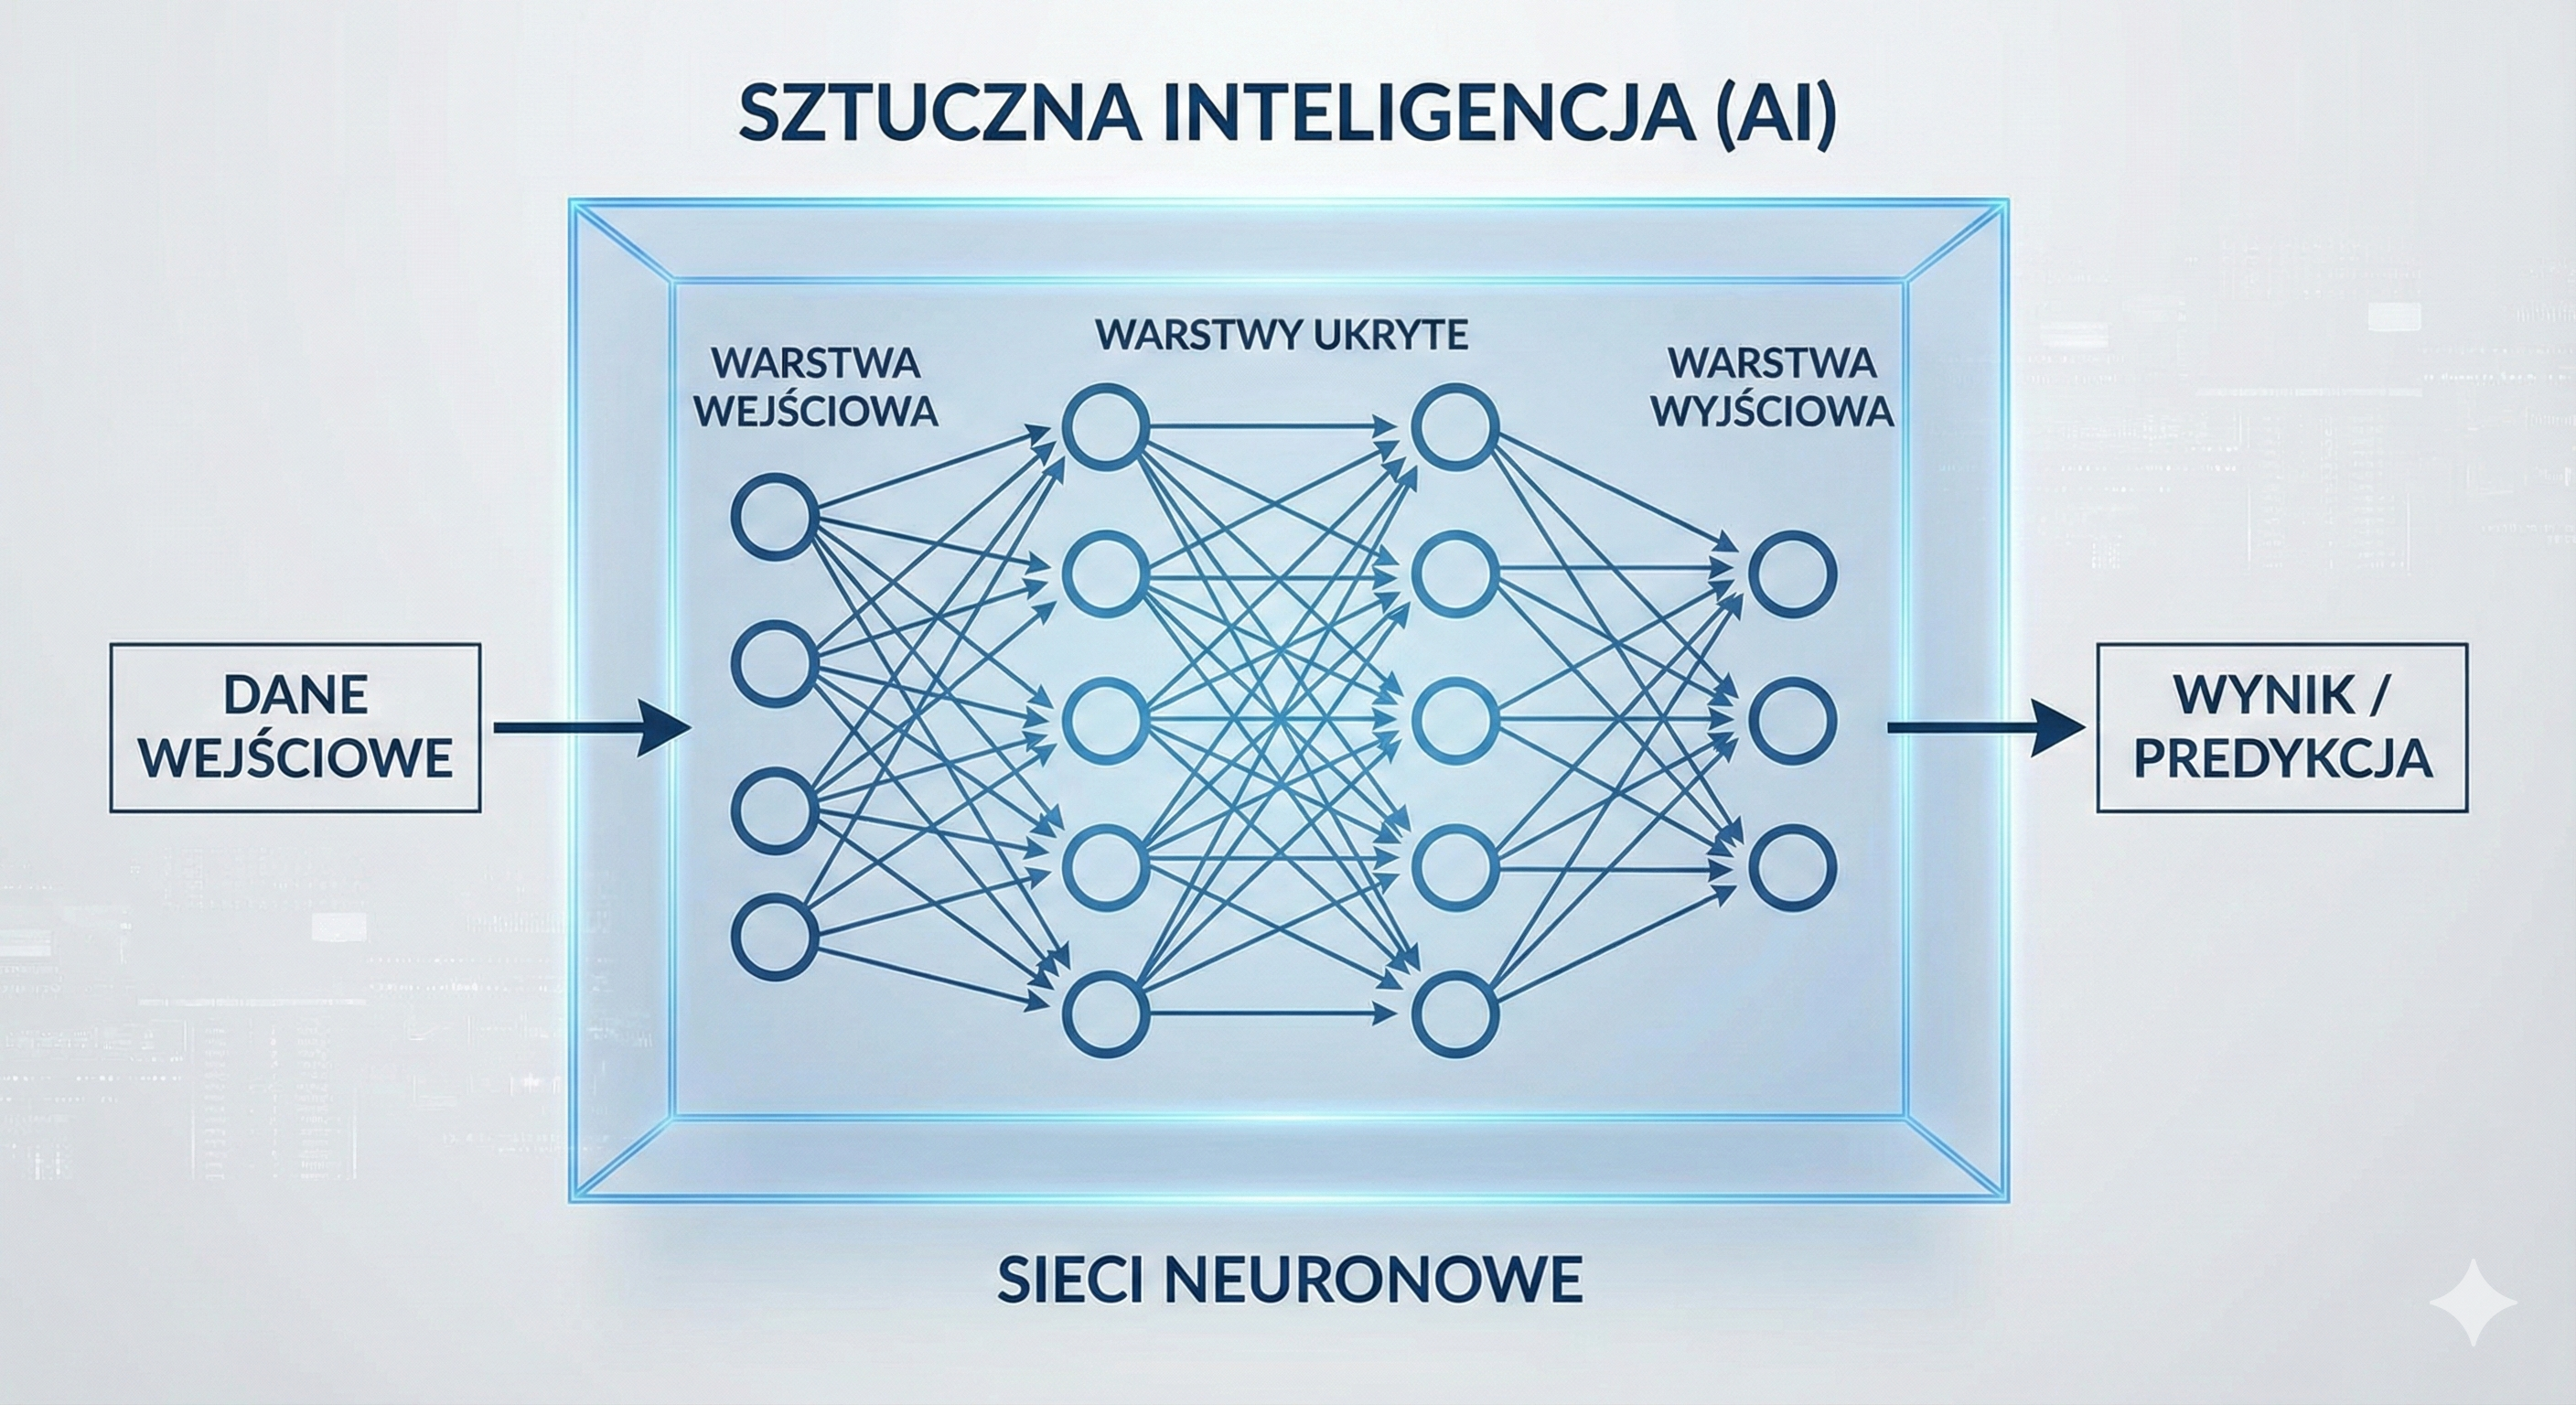
\includegraphics[width=0.9\textwidth]{obrazek.png}
    \caption{Schemat koncepcyjny sztucznej inteligencji i sieci neuronowych. Źródło: Obraz został wygenerowany za pomocą sztucznej inteligencji}
    \label{fig:siec}
\end{figure}

Jak podaje raport techniczny OpenAI, skalowanie tych modeli (zwiększanie ich rozmiaru i ilości danych) prowadzi do pojawienia się tzw. emergentnych zdolności, których nie przewidziano na etapie projektowania \cite{openai2023}. Oznacza to, że systemy te stają się coraz bardziej nieprzewidywalne, co rodzi nowe wyzwania w zakresie bezpieczeństwa AI.